\chapter[Processo de Design]{Processo de Design}

\section{Modelos de Ciclo de Vida}

Na área de interação humana-computador poucos modelos de ciclo de vida foram propostos, mas os que se destacam na literatura são: \textbf{modelo simplificado} proposto por Preece et. Al (2005), \textbf{modelo estrela} proposto por Hartson e Hix (1989) e o \textbf{modelo da engenharia de usabilidade} proposto por Mayhew (1999).

Cada ciclo tem a sua característica específica e de acordo com o contexto as suas atividades podem ser removidas ou adaptadas para um propósito específico.

\subsection{Ciclo de Vida em Estrela}
O modelo em estrela foi um dos primeiros voltados para IHC, e ele é composto por seis atividades, conforme ilustrado abaixo:

\begin{figure}[H]
	\centering
	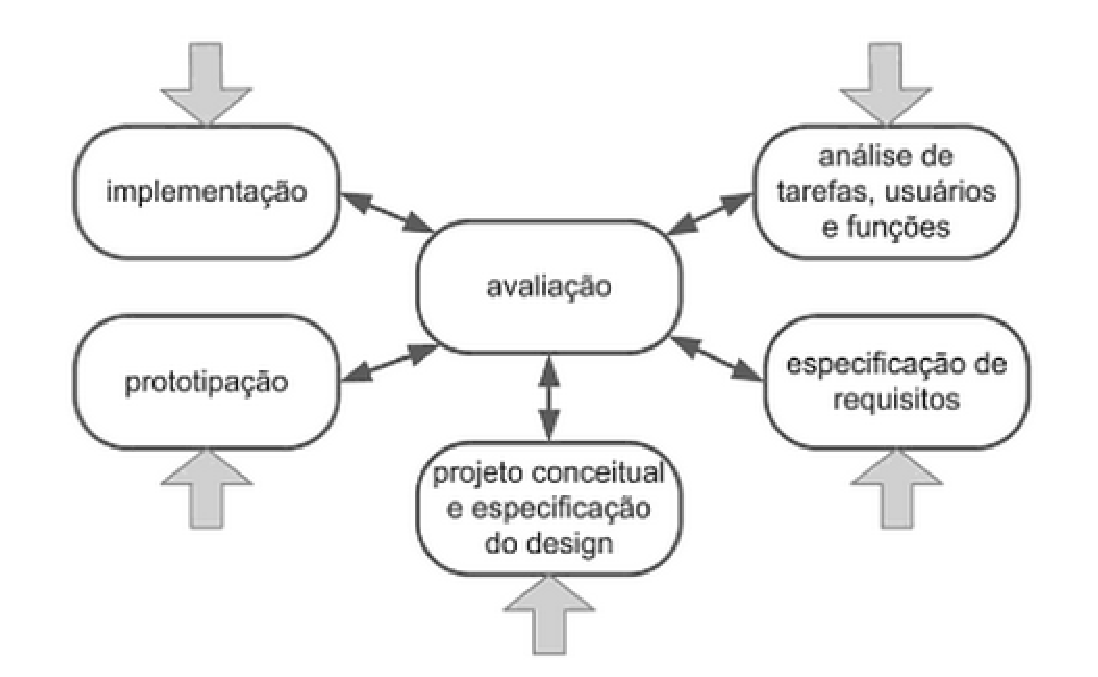
\includegraphics[scale=0.5]{figuras/modelo_estrela.eps}
	\caption{Ciclo de vida estrela}
\end{figure}

Algumas características são importantes de serem destacadas nesse modelo: a avaliação esta no centro das atividades e não existe ordenação de atividades, ou seja, o desenvolvimento pode iniciar em qualquer uma das atividades. 
\begin{itemize}
	\item \textbf{Análise de Tarefas de Usuário}: responsável pelo aprendizado da situação atual e pelo levantamento das necessidades e oportunidades de melhoria.
	\item \textbf{Especificação de Requisitos}: consolida uma interpretação da análise, definindo os problemas e necessidades que devem ser resolvidos com o projeto da solução.
	\item \textbf{Projeto Conceitual e Especificação do Design}: onde a solução de interação é concebida.
	\item \textbf{Prototipação}: versão interativa da proposta de solução são construidas para serem avaliadas.
	\item \textbf{Implementação}: onde o sistema interativo final é desenvolvido. Essa atividade em particular está fora do escopo do projeto, pois não se tem a intenção de desenvolver um sistema funcional.
	\item \textbf{Avaliação}: essa é a atividade central. Verifica se os dados coleta dos nas outras atividades de análise e dos requisitos estão de acordo. Deve, também, detectar problemas de usabilidade. Destaque importante para a avaliação, pois ela deve ser feita o enquanto ainda há tempo para corrigir os erros com o menor custo possível.
\end{itemize}



